We have implemented the proposed approach as a framework that provides the mechanisms and tools for deploying modular query engines, called Proteus.
Proteus consists of a collection of implementations of the QPU abstraction, as well as a service discovery mechanism that allows the QPU graph to self- organize with only local configuration input to each QPU.


\section{Query processing domain dissemination}

The set of queries that a query processing unit can process constitutes its query processing \textit{domain}.
As described in section~\ref{sec:qpc_tree},
we encode the query processing domain using a tree data structure, called domain tree.

The domain of a query processing unit depends on its functionality (class), its configuration, and, in most cases,
on the domains of its downstream connections as well.
This is because QPU classes such as Join and Partition Manager process a given query by breaking it down to sub-queries,
sending these sub-queries to their downstream connections,
and then performing a computation over the returned results.
Essentially, a QPU of this type de-composes queries into simpler tasks, and delegates some of these tasks to their downstream connections.
The set of queries that it can process, therefore, depends on the types of tasks that its downstream connections can perform.

Because of that, a query processing unit requires the domain tree of each of its downstream connections for its operation.
More specifically, as we described in section~\ref{sec:qpc_tree}, a QPU uses the downstream domain trees in order to:
(1) compute its own domain tree, and (2) generate downstream queries during query processing.
In this section, we describe the mechanism through which a query processing unit acquires the domain trees
of its downstream connections.

\subsection{Domain interface}
Query processing units expose an interface for sharing their domain tree:

\begin{displaymath}
  GetDomain() \rightarrow [(QPUClass, DomainTree)]
\end{displaymath}

An invocation of $GetDomain$ returns a stream that contains $DomainTree$ records, where $DomainTree$ is a serialization of a domain tree.
When a QPU receives an invocation of its domain interface, it establishes an output stream with the caller,
and sends a $DomainTree$ records, which represents its domain tree.
Each time there is a change to its domain tree, the QPU sends an additional $DomainTree$ record through the stream,
representing the updated domain tree.

Similarly to the query interface, an edge in the edge in the QPU graph between $Q_A$ and $Q_B$ indicates that $Q_A$ can
invoke the domain interface of $Q_B$.

\medskip
\noindent
We design the domain interface response as a stream rather that an one-time response in order to enable propagation of
configuration, domain and topology changes through the QPU graph.
This is a first step towards enabling \textit{dynamic reconfiguration} of QPU architectures.
Example of dynamic reconfiguration might include the creation new indexes or materialization of view at runtime.
We consider dynamic reconfiguration of QPU architecture out of the scope of this work.
It is, however, a direction for future work.

\subsection{Query processing domain initialization}

The first task of the constructor of each query processing unit class is to initialize the QPU's domain tree.
For the Corpus Driver class this is performed using the input configuration (section \todo{}).
Every other QPU class, as discussed above, requires the domain trees of its downstream connections in order to compute its own domain tree.
Because of that, the constructor method of every QPU class except of the Corpus Driver starts by sending a $GetDomain$ request to each
of its downstream connections.
After receiving the corresponding responses, the constructor computes the QPU's domain tree, using the rules presented in section \todo{domain init rules}.

If a QPU receives a $GetDomain$ request while still this process is being performed, it creates the response stream,
and sends the first response to the stream as soon it computes its domain tree.

We illustrate this process using the QPU shown in Figure~\ref{fig:domain_example_graph} as an example.
Figure~\ref{fig:domain_sequence_diag} depicts a sequence diagram that describes the message exchanges between QPUs in the graph
for initializing their query processing domains.
Upon initialization, the $Join$, $Selection_1$ and $Selection_2$ send a $GetDomain$ request to each of their downstream
connections,
while the $Corpus$ $Driver_1$ and $Corpus$ $Driver_2$ compute their query processing domains using their input configuration.
Once each $Corpus$ $Driver$ QPU computes its domain tree, it responds to the corresponding $GetDomain$ request.
When each $Selection$ QPU receives the $GetDomain$ response, it calculates its domain tree, and then it responds to the request from $Join$.
Finally, $Join$ receives the responses from $Selection_1$, $Selection_2$, and computes its domain tree.

\medskip
\noindent
The goal of the domain dissemination mechanism is to reduce the input configuration required by QPU instances,
in order to simplify the process of configuring and deploying a QPU architecture.
Thanks to this mechanism, the configuration of a query processing unit consists of ``local'' configuration
(configuration about that specific QPU), as well as the endpoints of its downstream connections.
The QPU can then use domain interface of its connections to obtain information about them.

\begin{figure}
    \centering
    \begin{minipage}{.3\textwidth}
        \centering
        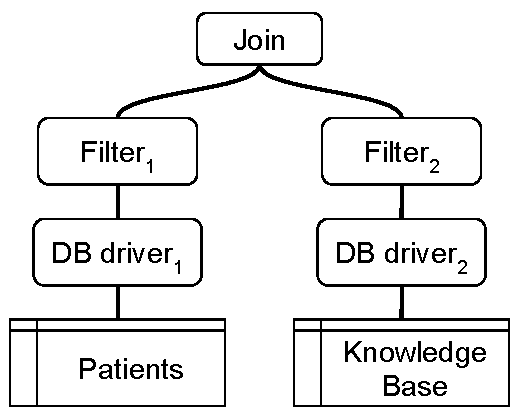
\includegraphics[scale=0.5]{./figures/design_pattern/qpu_graph_emergent_properties.pdf}
        \caption{}
        \label{fig:domain_example_graph}
    \end{minipage}%
    \begin{minipage}{.7\textwidth}
        \centering
        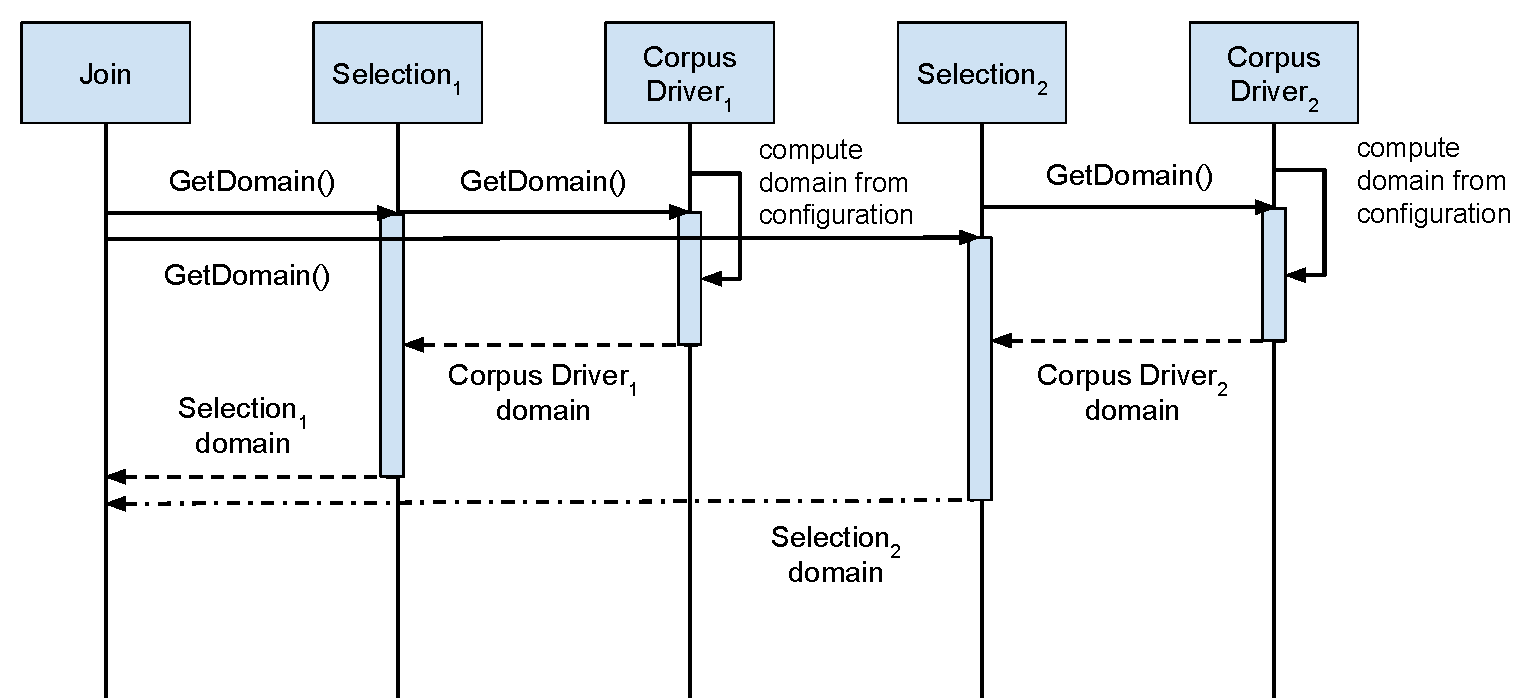
\includegraphics[scale=0.4]{./figures/proteus/domain_sequence_diag.pdf}
        \caption{}
        \label{fig:domain_sequence_diag}
    \end{minipage}
\end{figure}



\section{Query processing unit service}

Proteus provides an implementation of the query processing architecture presented in chapter \todo{ref chapter 5}.
In Proteus, the query processing unit component is implemented as a service, i.e. a daemon process.
In this section we describe the system design and architecture of Proteus' query processing unit service.

\medskip
\noindent
The QPU service design is guided by the principles of the query processing unit model.
Instead of implementing a separate QPU service for each QPU class,
we design the query processing unit service as a \textit{polymorphic} service:
Different instances of the same service implement different QPU classes, based on their configuration.
To achieve that, we separate the components that are common to every QPU class, such as the configuration and query processing domain
component,
and the components that are class-specific.
For the class-specific components, we provide implementations for different classes in the form a library.
We ensure that components are separated and communicate though well-defined APIs.

Our goal with this design is to make the query processing service \textit{extensible}.
Implementing an additional QPU class consists of defining the 

\begin{figure}
  \centering
    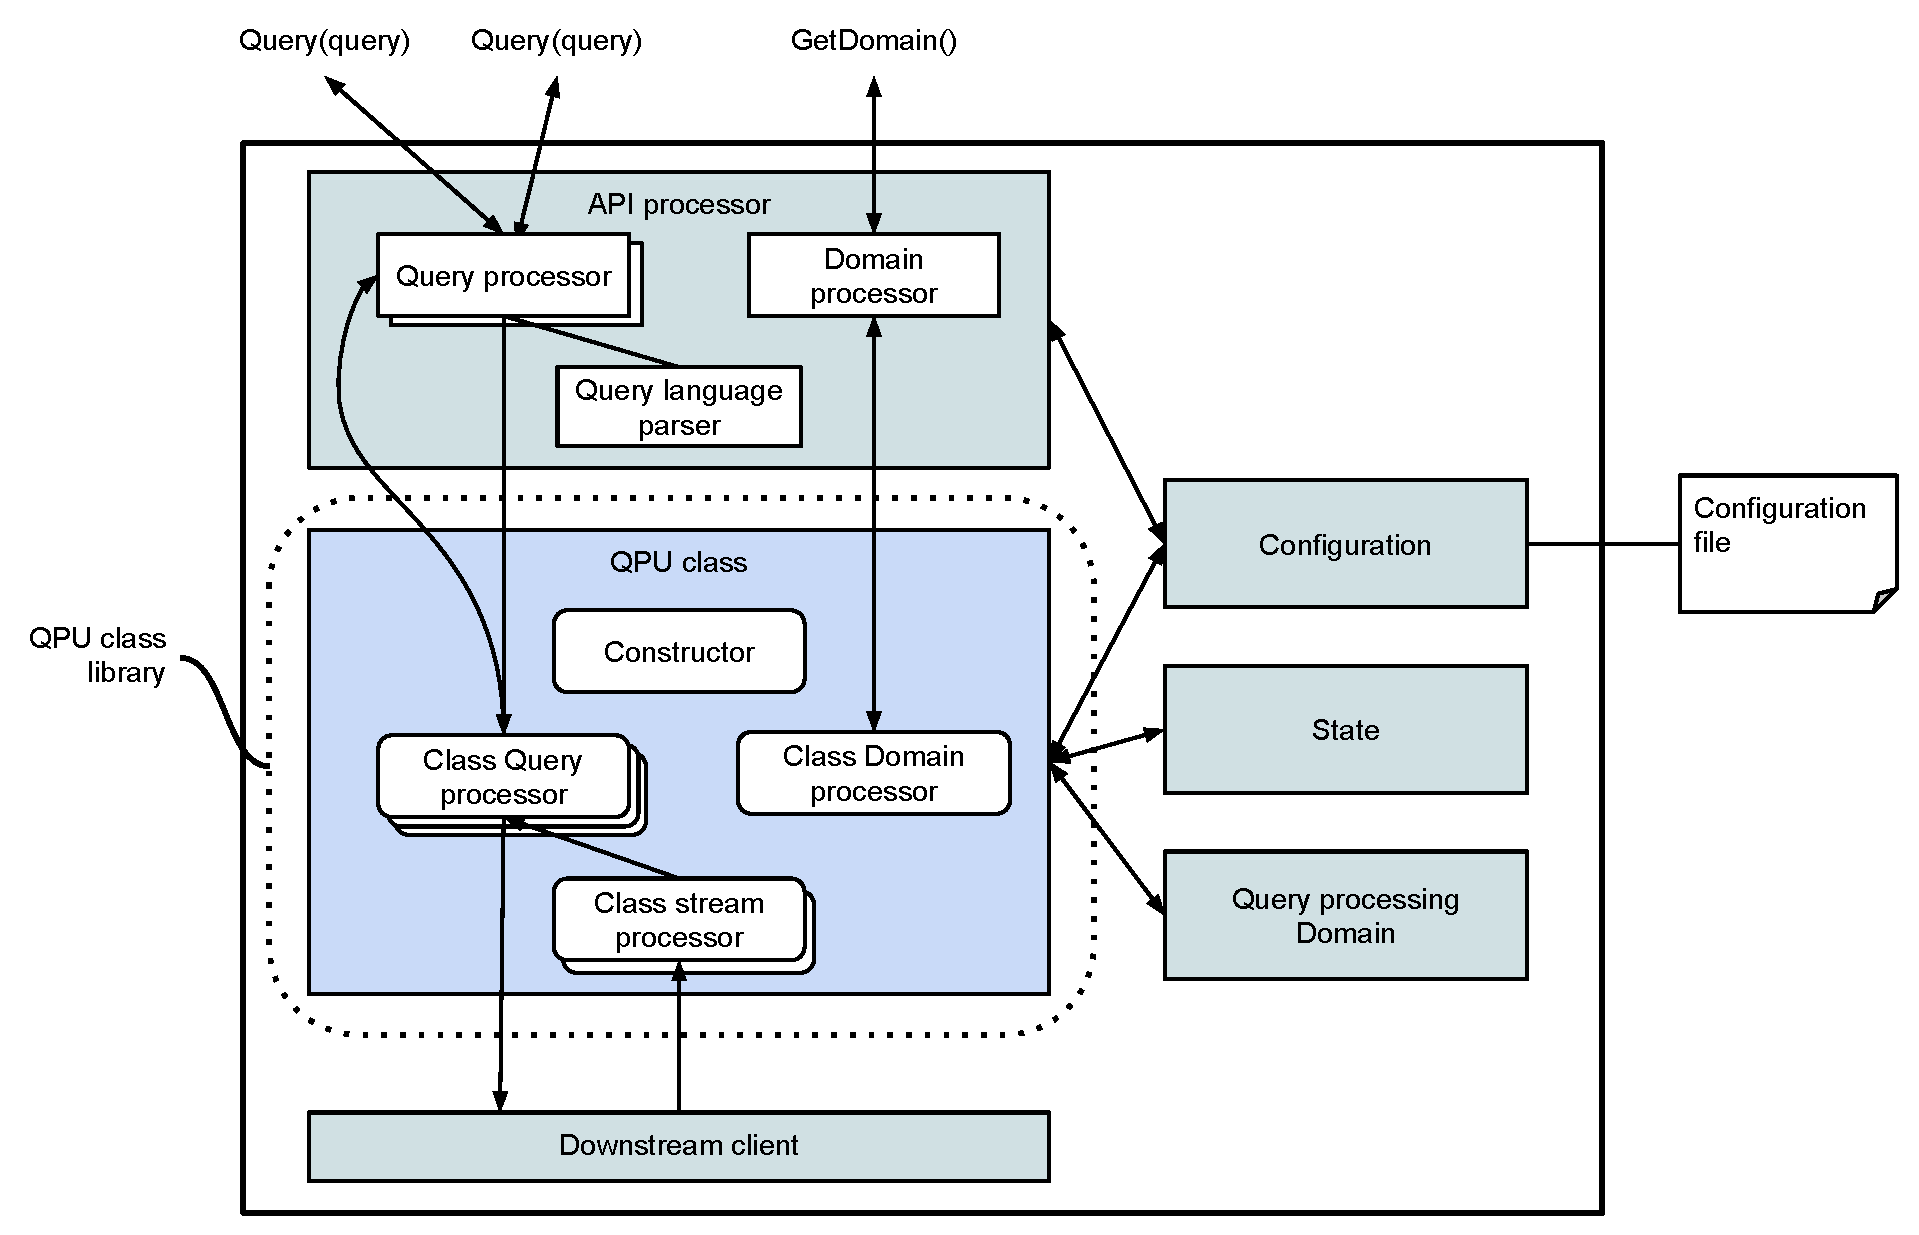
\includegraphics[width=0.7\textwidth]{./figures/proteus/QPU_architecture.pdf}
  \caption{QPU architecture  ...}
  \label{fig:qpu_arch}
\end{figure}


\medskip
\noindent
Figure \ref{fig:qpu_arch} depicts the components of the query processing unit service.

The \textbf{QPU Class Library} contains a set of QPU class definitions.
Each QPU class definition consists of three \textit{method} definitions,
which are the QPU methods described in section \todo{}: constructor, query processor, input processor.

The \textbf{API Processor} is responsible for receiving and processing incoming requests for the two open interfaces of
the query processing unit:
the query and the domain interface.
When it receives a query request,
the API Processor first parses the given query to a query parse tree \todo{ref} using the Query Language Parse.
If the query parse tree is successfully created, the API Processor creates initiates a response stream,
and spawns an instance of the Class Query Processor of the QPU class specified in the configuration.
The Class Query Processor sends query result records back to the API Processor which emits them as output stream records.

Similarly, when the API processor receives a GetDomain request,
it spawns an instance of the Class Domain processor, and emits the each received response as a stream record.

The API Processor can process multiple query and GetDomain requests concurrently.
For each received request, it creates a new output thread, and spawns a new instance of the corresponding QPU class method.


The \textbf{State} component provides any API that other components can use for storing and retrieving state.
It is used by derived state QPU classes, such as the Index and Materialized View classes, for storing their
derived state structures.
The QPU design defines only the API of the State component in order to enable the component's implementation to be modular.
We have implemented three versions of the State component: an in-memory implementation using an ordered map data structure,
one using the MySQL \todo{ref}, and one using AntidoteDB \todo{ref}


A configuration file is passed to the QPU service during initialization.
The \textbf{Configuration} component is responsible for parsing the configuration file into a set of configuration parameters.
It exposes an API that other components can use to retrieve configuration parameters.
Configuration parameters include:

\begin{itemize}
  \item The QPU service's class.
  \item The endpoints of the QPU service's connections.
  \item Class specific configuration.
  While presenting an exhaustive list of the configuration parameters of each QPU class is out of the scope of this
  section, we present a few examples below.

  For the Corpus Driver class, the configuration specifies the endpoint of the corpus data,
  the table it is responsible for, and, optionally, the table's schema.

  For the Index class, as described in section \todo{ref case study 1} the configuration specifies an attribute name
  and an interval of values for that attribute.
  The Index QPU is responsible for  for the indexed attribute.

  For the Aggregator class, the configuration specifies an aggregator
\end{itemize}



\section{Configuration language}

In this section, we present a simple language for describing QPU-based query processing architectures.

The goal of a program written in the language is to describe a QPU graph
--- the class and configuration of the QPUs at its vertices, and the connections among them ---
and the placement of the graph vertices across system nodes.

A Proteus program comprises a series of placement context assignments,
a series of QPU instance declarations, and a series of declarations of connections between QPU instances.

A placement context is node or collection of nodes.
A placement context assignment has the following syntax:

\begin{lstlisting}[
          showspaces=false,
          basicstyle=\ttfamily,
          commentstyle=\color{gray},
          rulecolor=\color{black},
          stringstyle=\color{mymauve},
          frame=L,
          xleftmargin=\parindent
        ]{}
PlacementCtx([endpoint], ContextName)
\end{lstlisting}

\noindent
where $[endpoint]$ is a collection of system nodes, expressed as hostnames, or IP addresses,
and $ContextName$ is the name of the context assigned to these nodes.
For example, the program:

\begin{lstlisting}[
          showspaces=false,
          basicstyle=\ttfamily,
          commentstyle=\color{gray},
          rulecolor=\color{black},
          stringstyle=\color{mymauve},
          frame=L,
          xleftmargin=\parindent
        ]{}
PlacementCtx([10.200.4.56], "node_1")
PlacementCtx([10.200.3.45], "node_2")
PlacementCtx([10.200.4.56, 10.200.3.45], "dc_eu")
\end{lstlisting}

\noindent
assigns the context ``node\_1'' to the node with address 10.200.4.56,
the context ``node\_2'' to  the node with address 10.200.3.45 ,
and the context ``dc\_eu'' to both nodes.

\medskip
\noindent
A QPU context declaration has the following syntax:


% \section{Fault tolerance}
% Describe the mechanisms provided by Proteus for tolerating faults during query
% processing.
% \begin{itemize}
%   \item Lost or re-ordered stream records.
%   \item Mid-query QPU crash.
%   \item Partitions.
% \end{itemize}

% \section{Implementation}
% Report on the implementation of different components of Proteus, including:
% \begin{itemize}
%   \item The framework used for communication between QPUs.
%   \item How streams are implemented.  
%   \item ...
% \end{itemize}

\section{Implementation}

Driver

connection pool

thread pool